\documentclass[12pt]{article}
\linespread{1.2}
\usepackage[margin=2cm]{geometry}
\usepackage[utf8]{inputenc}
\usepackage{amsfonts}
\usepackage{amsmath}
\usepackage{multicol}
\usepackage{amsthm}
\usepackage{amssymb,scrextend}
\usepackage{graphicx,tikz}
\newtheorem{dfn}{Definition}
\renewcommand{\qed}{\hfill$\blacksquare$}
\let\newproof\proof
\renewenvironment{proof}{\vspace{1em}\begin{addmargin}[2em]{0em}\begin{newproof}}{\end{newproof}\end{addmargin}\qed}
\newenvironment{theorem}[2][Theorem]{\begin{trivlist}
\item[\hskip \labelsep {\bfseries #1} \hskip \labelsep {\bfseries #2.}]}{\end{trivlist}}
\newenvironment{example}[2][Example]{\begin{trivlist}
\item[\hskip \labelsep {\bfseries #1} \hskip \labelsep {\bfseries #2.}]}{\end{trivlist}}
\newenvironment{lemma}[2][Lemma]{\begin{trivlist}
\item[\hskip \labelsep {\bfseries #1} \hskip \labelsep {\bfseries #2.}]}{\end{trivlist}}
\newenvironment{exercise}[2][Exercise]{\begin{trivlist}
\item[\hskip \labelsep {\bfseries #1} \hskip \labelsep {\bfseries #2.}]}{\end{trivlist}}
\newenvironment{problem}[2][Problem]{\begin{trivlist}
\item[\hskip \labelsep {\bfseries #1} \hskip \labelsep {\bfseries #2.}]}{\end{trivlist}}
\newenvironment{corollary}[2][Corollary]{\begin{trivlist}
\item[\hskip \labelsep {\bfseries #1} \hskip \labelsep {\bfseries #2.}]}{\end{trivlist}}
\usepackage{fancyhdr,enumitem,changepage,url}
\pagestyle{fancy}
\author{Warren Atkison}
\date{\today}
\setlength{\headheight}{15pt}
\begin{document}
\fancyhf{}
\fancyhead[L]{Warren Atkison}
\fancyhead[C]{Exam 1}
\fancyhead[R]{\today}
\fancyfoot[R]{\thepage}

\begin{problem}{2}
	Let $n,p,q$ be positive integers so that $p\le n$ and $q \le n$. Prove that
	\[
		\binom{n}{p} \binom{n}{q} = \sum_{k=0}^n \binom{n}{k} \binom{n-k}{p-k}\binom{n-p}{q-k}
	\]
\end{problem}
\begin{proof}
	We shall prove this combinatorially,
	\begin{itemize}
		\item[\textbf{LHS:}] from a set of $n$ elements, choose a subset of $p$ elements $A$, and a subset of $q$ elements $B$.
		\item[\textbf{RHS:}] from a set of $n$ elements choose $k$ people to be in both subsets. Of the $n-k$ elements left over, choose $p-k$ elements to be apart of the first subset, for a total of $p$ elements in the subset. From the $n-p$ elements left after choosing the first subset (the $k$ elements in both are also accounted for when subtracting $p$), choose $q - k$ elements to be in the second subset for a total of $q$ elements in that subset. Do this for $0 \le k \le n$. We are left with all ways to choose two subsets, one of $p$ elements one of $q$ elements. 
	\end{itemize}
	\begin{center}		
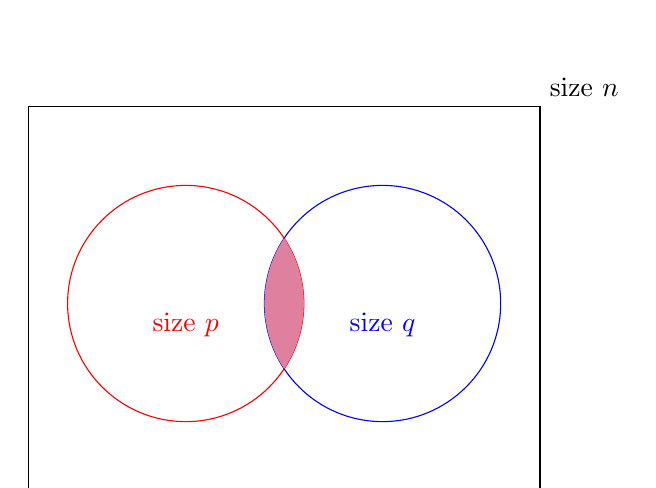
\begin{tikzpicture}
  % Box
	\draw (-2,-2.5) rectangle (4.5,2.5) node[above right] {size $n$};
  
  % Circles
	\draw[red] (0,0) circle (1.5cm) node[align=center, below] {size $p$};
	\draw[blue] (2.5,0) circle (1.5cm) node[align=center, below] {size $q$};
  
  % Labels
  \node at (1.25,1.5) {};
  \node at (-0.75,-2) {};
  \node at (3.75,-2) {};
  
  % Intersection
  \begin{scope}
    \clip (0,0) circle (1.5cm);
    \fill[purple!50] (2.5,0) circle (1.5cm);
  \end{scope}
\end{tikzpicture}
	\end{center}
	The LHS is the number of ways to choose two subsets, one of size $p$ and one of size $k$, from a set $n$ with replacment of elements from $n$. The RHS counts the number of wasy to choose these two subsets by filling the intersection of the two subsets first, then filling the rest of the the two subsets from the elements not yet in a subset (without replacment from $n$).
\end{proof}
\begin{problem}{9}
	A patient is in the hospital recovering from serious surgery and her physician wants her to increase her exercise gradually. On the first day she is allowed to walk to the cafeteria. On the second day two walks, etc. If the patient stays for $n$ days and makes $3$ total walks to the cafeteria, how many ways is this possible? What about $k$ walks?
\end{problem}
In the first case, the most we can walk is 3 times in a day, so
\[
	x_1 + x_2 + x_3 + \ldots + x_n = 3
\]
where $x_1 \le 1$, $x2 \le 2$, $x_i \le 3$ for $3 \le i \le n$. The generating function for this is as follows
\begin{align*}
	\left(\frac{1}{1-x} - \frac{x^2}{1 - x}\right)\left(\frac{1}{x-1} - \frac{x^3}{1 - x}\right)\left(\frac{1}{1-x}-\frac{x^4}{1-x}\right)^{n-2}
\end{align*}
Which can be simplified to
\begin{align*}
	(1 + x)(1 + x + x^2)(1 + x + x^2 + x^3)^{n-2} &= (x^3 + 2x^2 + 2x + 1)(1 + x + x^2 + x^3)^{n-2} \\
						      &= (x^3 + 2x^2 + 2x + 1)\left(\sum_{|\alpha| = n-2} \binom{n-2}{\alpha}x^{\alpha}\right)
\end{align*}
where $\alpha = (\alpha_1,\alpha_2,\alpha_3,\alpha_4)$ for $0 \le \alpha_i \le n-2$ and
\[
	x^{\alpha} = 1^{\alpha_1}\cdot x^{\alpha_2}\cdot x^{2\alpha_3} \cdot x^{3\alpha_4} = x^{\alpha_2 + 2\alpha_3 + 3\alpha_4}.
\]
Now we want to find when $\alpha_2 + 2\alpha_3 + 3\alpha_4 = 3,2,1,0$. For 3 we have $(\alpha_2 = 3)$, $(\alpha_2 = 1, \alpha_3 = 1)$, and $(\alpha_4 = 1)$, for 2 we have $(\alpha_2 = 2)$, $(\alpha_3 = 1)$, for 1 we have $(\alpha_2 = 1)$, and for zero they are all zero. Remembering $\alpha_1 + \alpha_2 + \alpha_3 + \alpha_4 = n - 2$ in our sum, we can determine $\alpha_1$ for our multinomials. So
\begin{align*}
	\sum_{|\alpha| = n-2} \binom{n-2}{\alpha}x^{\alpha} &= 1 + \binom{n-2}{n-3,1,0,0}x + \left[\binom{n-2}{n-4,2,0,0} + \binom{n-2}{n-3,0,1,0}\right]x^2 \\
							    &+ \left[\binom{n-2}{n-5,3,0,0} + \binom{n-2}{n-4,1,1,0} + \binom{n-2}{n-3,0,0,1}\right]x^3 + \ldots.
\end{align*}
Multiplying by $(x^3 + 2x^2 + 2x + 1)$ and only looking for the $x^3$ coeffecient we get
\begin{align*}
	C_3 &= 1 + 2\left(\frac{(n-2)!}{(n-3)!}\right) + 2\left(\frac{(n-2)!}{(n-4)!2!} + \frac{(n-2)!}{(n-3)!}\right) + \frac{(n-2)!}{(n-5)!3!} + \frac{(n-2)!}{(n-4)!} + \frac{(n-2)!}{(n-3)!} \\
	    &= 1 + 2(n-2) + 2\left(\frac{(n-2)(n-3)}{2!}+(n-2)\right) + \frac{(n-2)(n-3)(n-4)}{6} + (n-2)(n-3) + (n-2) \\
	    &= 1 + 5(n-2) + 2(n-2)(n-3) + \frac{(n-2)(n-3)(n-4)}{6} \\
	    &= 1 + 5n - 10 + 2(n^2 - 5n + 6) + \frac{n^3 - 9n^2 + 26n - 24}{6} \\
	    &= 1 + 5n - 10 + 2n^2 - 10n + 12 + \frac{n^3}{6} - \frac{3n^2}{2} + \frac{13n}{3} - 4 \\
	    &= \frac{n^3}{6} + \frac{n^2}{2} - \frac{2n}{3} - 1
\end{align*}
\end{document}
